\section{Diseño y Ensamblado}
\frame{
	\ifdebug
	\frametitle{Outline\hfill{\color{red} \emph{M}}}
	\else
	\frametitle{Outline}
	\fi
	\tableofcontents[currentsection]
	}

\subsection*{PyID}
% Una subsection* crea un nuevo "grupo de puntos"

\frame{
	\ifdebug
	\frametitle{P\&ID\hfill{\color{red} \emph{M}}}
	\else
	\frametitle{P\&ID}
	\fi

	\begin{center}
		\textbf{Diagrama de Tuberías e Instrumentación}
		\vspace{0.25cm}
		
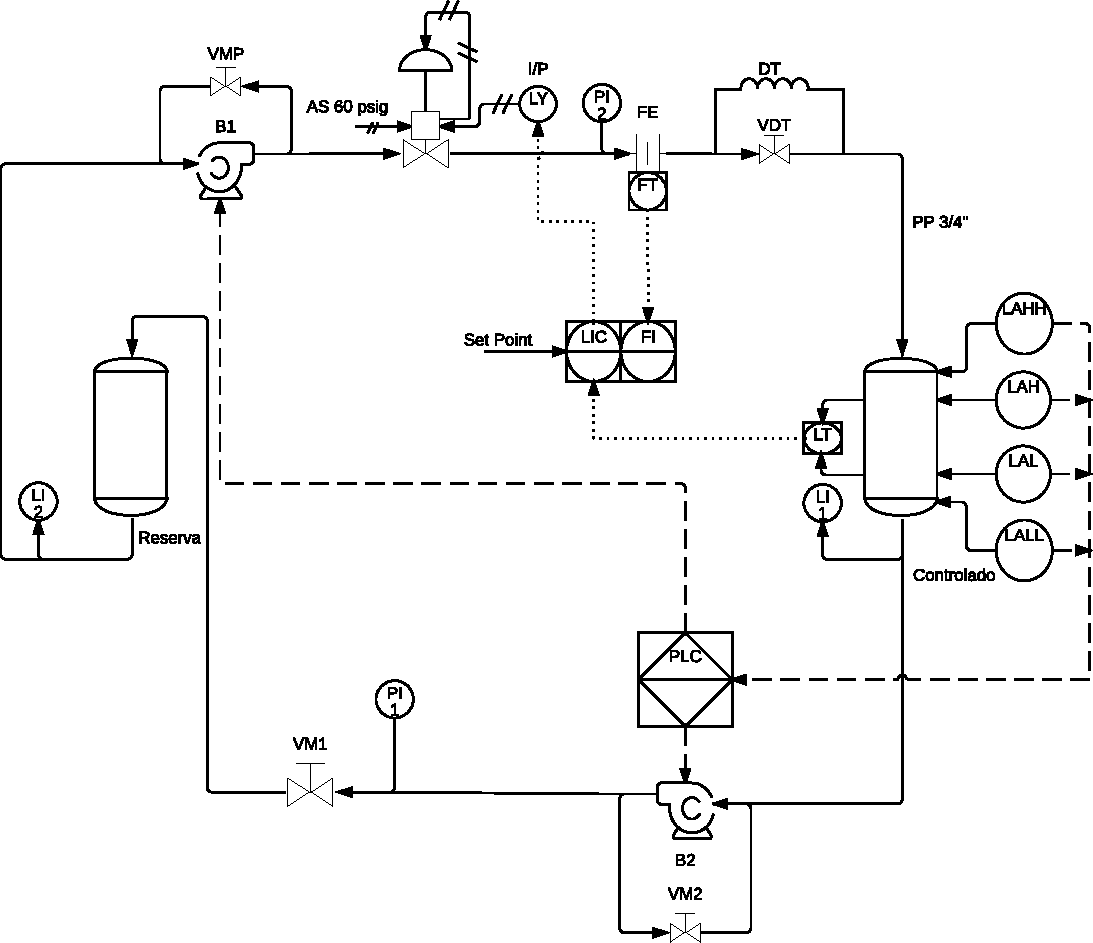
\includegraphics[width=6.5cm]{Sections/2-DisenoEnsamblado/Images/pyid60-1.pdf}
	\end{center}
	\vspace{-.5cm}
	\begin{itemize}
		\item {\color{newcolor} Codificación}:
		\begin{itemize}
			\item Primer letra: designa la variable medida o de
			interés
			\item Letras siguientes: designa la función del
			componente
		\end{itemize}
	\end{itemize}
	
}


\subsection*{Circuito hidráulico}
\frame{
	\ifdebug
	\frametitle{Tuberías y Tanques\hfill{\color{red} \emph{M}}}
	\else
	\frametitle{Tuberías y Tanques}
	\fi


	\begin{columns}[t]
		\begin{column}{0.63\textwidth}
			\begin{center}
				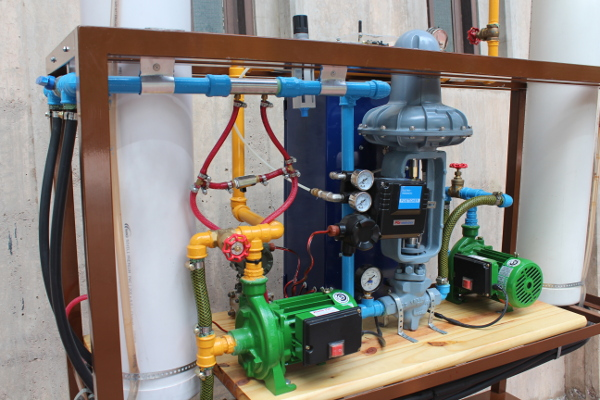
\includegraphics[height=4.5cm]
{Sections/2-DisenoEnsamblado/Images/caneria1.JPG}
			\end{center}
			\begin{itemize}
				\item {\color{newcolor} Tuberías}:
				\begin{itemize}
					\item Rígidas
					\item Semi rígidas
					\item Flexibles
				\end{itemize}
			\end{itemize}
		\end{column}
		\begin{column}{0.37\textwidth}
			\begin{center}
				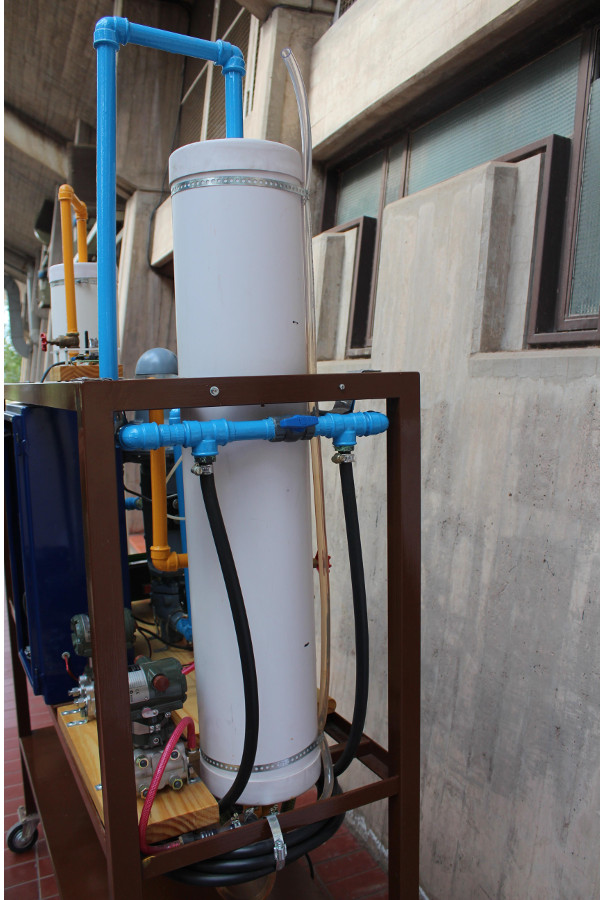
\includegraphics[height=4.5cm]
{Sections/2-DisenoEnsamblado/Images/caneria2.JPG}
			\end{center}
			\begin{itemize}
				%\vspace{0.25cm}
				\item {\color{newcolor} Tanques}:
				\begin{itemize}
					\item Reservorio
					\item Controlado
				\end{itemize}
			\end{itemize}
		\end{column}
	\end{columns}
}

\frame{
	\ifdebug
	\frametitle{Flujo de Agua\hfill{\color{red} \emph{M}}}
	\else
	\frametitle{Flujo de Agua}
	\fi

	\textbf{Bombas}
	
	\vspace{.25cm}
	
	{\color{newcolor} Objetivo:} generar un flujo de agua ininterrumpido
	entre el reservorio y el tanque controlado.
	
	\vspace{.25cm}

	\begin{columns}
	 \begin{column}{.35\textwidth}
	 Bombas centrífugas funcionando ininterrumpidamente
	 \end{column}
	 \begin{column}{.65\textwidth}
	 \begin{center}
	  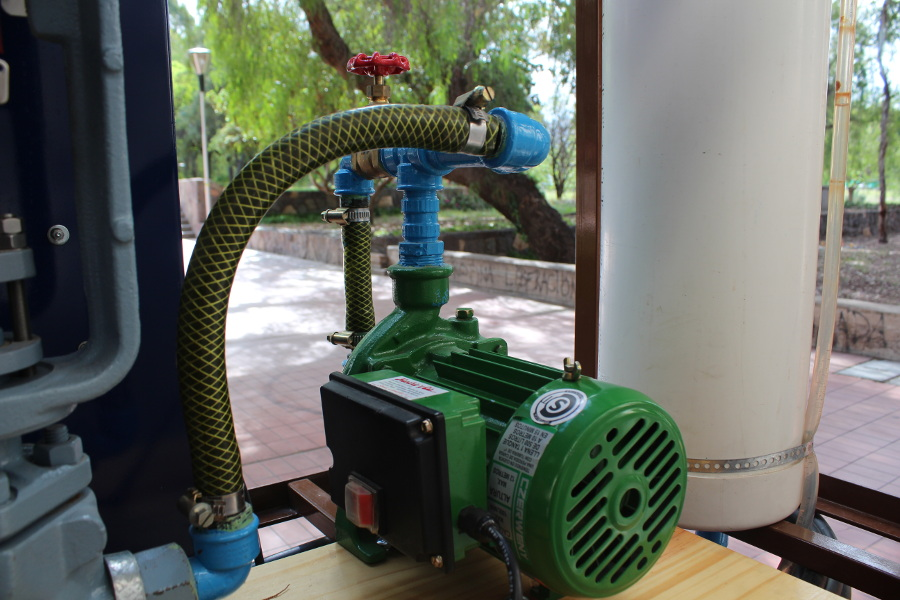
\includegraphics[width=\textwidth]
	  {Sections/2-DisenoEnsamblado/Images/bomba.JPG}
	  
	  \footnotesize
	  Detalle bomba \texttt{B1}
	  \end{center}
	 \end{column}
	\end{columns}
}
\subsection*{Válvula globo, con servoactuador de diafragma - resorte}
\frame{
	\ifdebug
	\frametitle{Válvula globo con servoactuador de diafragma - 
resorte\hfill{\color{red} \emph{F}}}
	\else
	\frametitle{Válvula globo con servoactuador de diafragma - resorte}
	\fi

	\textbf{Generalidades}

	\vspace{0.25cm}
	Elemento central en la planta, efectúa las acciones de control

	\begin{center}
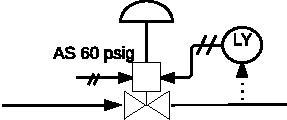
\includegraphics[scale=1]{Sections/2-DisenoEnsamblado/Images/ValvPyID.pdf}
	\end{center}
	\vspace{-0.25cm}
	\begin{columns}[t]
		\begin{column}{0.5\textwidth}
			\begin{itemize}
				\item {\color{newcolor} Características}:
				\begin{itemize}
					\item Válvula Isoporcentual
					\item Aire para abrir (NC)
					\item Con electroposicionador
				\end{itemize}
			\end{itemize}
		\end{column}
		\begin{column}{0.5\textwidth}
			\begin{itemize}
				\item {\color{newcolor} Entradas}:
				\begin{itemize}
				 \item Aire: $4\,bar$
				 \item Señal: $4$ - $20\,mA$
				\end{itemize}
			\end{itemize}
		\end{column}
	\end{columns}
}

\frame{
	\ifdebug
	\frametitle{Válvula globo con servoactuador de diafragma - 
resorte\hfill{\color{red} \emph{F}}}
	\else
	\frametitle{Válvula globo con servoactuador de diafragma - resorte}
	\fi

	\textbf{Principio de Funcionamiento}
	\begin{columns}[t]
		\begin{column}{0.5\textwidth}
		\begin{center}
		 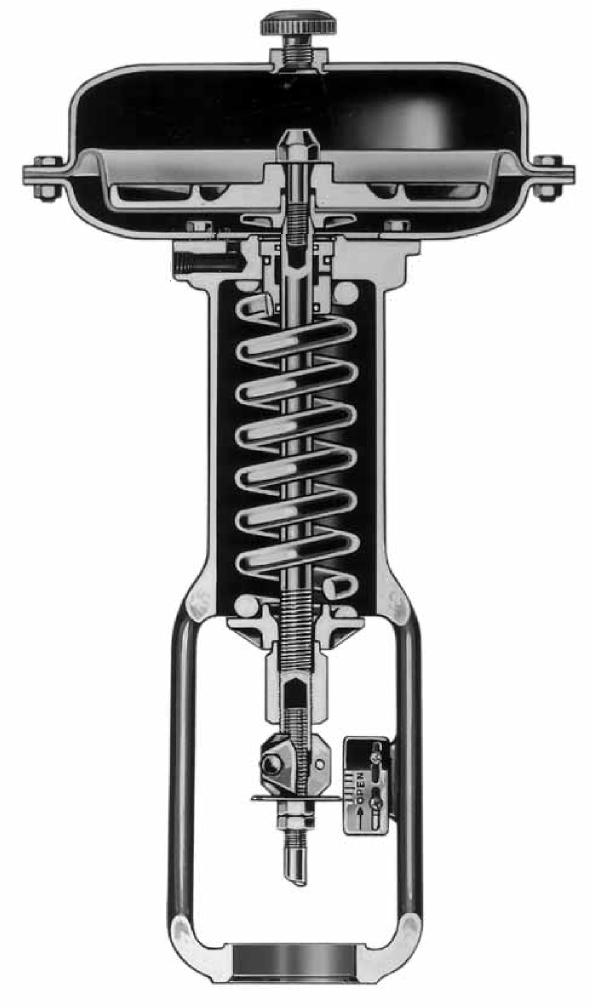
\includegraphics[width=.6\textwidth]
{Sections/2-DisenoEnsamblado/Images/ActuadorValvNeum.png}
 \footnotesize
 
       Actuador Neumático Inverso
		\end{center}


		\end{column}

		\begin{column}{0.5\textwidth}
		
		\begin{center}
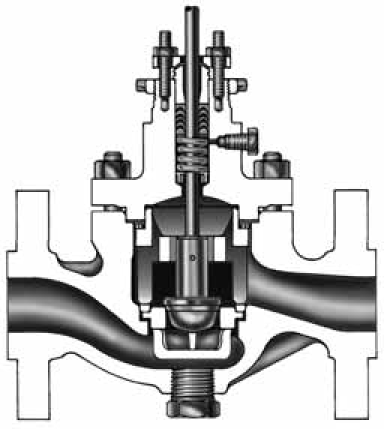
\includegraphics[width=.6\textwidth]
{Sections/2-DisenoEnsamblado/Images/ValvGlob.png}

 \footnotesize
       Cuerpo de la válvula
       
       Conjunto asiento-obturador
\end{center}
		\begin{itemize}
		 \item Convertidor I/P, presión de aire comprimido ($3$ - 
$15\,psi$)
		\item Equilibrio presión aire - resorte
		\end{itemize}
		\end{column}

	\end{columns}
}
\frame{
	\ifdebug
	\frametitle{Válvula globo con servoactuador de diafragma - 
resorte\hfill{\color{red} \emph{F}}}
	\else
	\frametitle{Válvula globo con servoactuador de diafragma - resorte}
	\fi
	\begin{center}
	 	\textbf{Curvas características}
	\end{center}
	\vspace{0.25cm}
	\begin{columns}[t]
		\begin{column}{0.5\textwidth}
		\textbf{Caract. caudal inherente}
		
		Relaciona carrera-caudal, a $\Delta p$ cte.
		\begin{center}
		 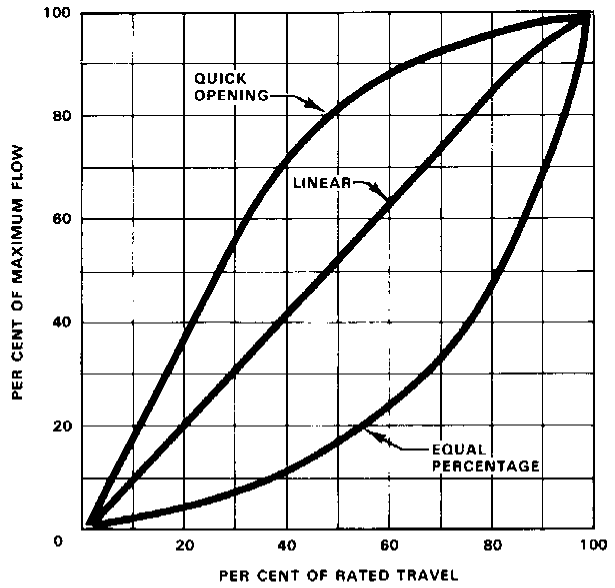
\includegraphics[width=.9\textwidth]
{Sections/2-DisenoEnsamblado/Images/Inherente.png}
 \footnotesize
		\end{center}
% 		\begin{itemize}
% 		 \item Lineal
% 		 \begin{align*}
% 		  q = k\,l
% 		 \end{align*}
% 		 \item Isoporcentual
% 		 \begin{align*}
% 		  \dfrac{q_{max}}{q_{min}} = e^a
% 		 \end{align*}
% 		 \item Quick Opening
% 		\end{itemize}


		\end{column}

		\begin{column}{0.5\textwidth}
		\textbf{Caract. caudal efectiva}
		
		Idem, a $\Delta p$ variable
		
		\begin{align*}
	 q_e &= \dfrac{1}{\sqrt{1-r+\dfrac{r}{{q_i}^2}}}
	\end{align*}
	
			\vspace{-.6cm}
	
	\begin{figure}[ht]
  \centering
  \resizebox {\columnwidth} {!} {
  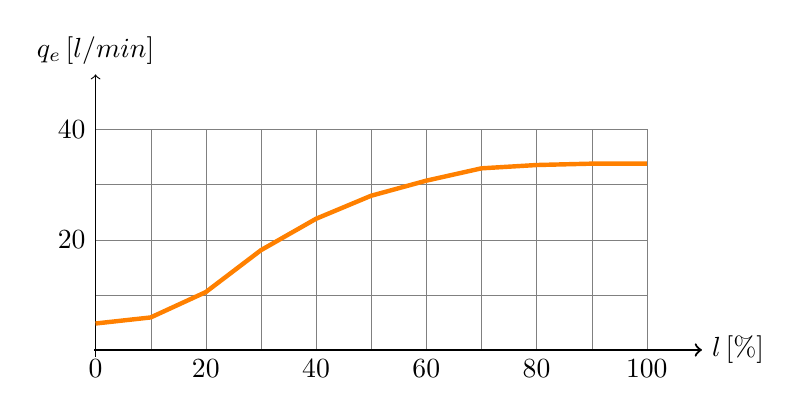
\begin{tikzpicture}[scale=.07,domain=0:110]
    
    \draw[ultra thin,color=gray,step=10cm] (100,40) grid (0.1,0.1);
    \draw[thick,->] (-0.2,0) -- (110,0) node[right,draw=none] {$l\,[\%]$};
    \draw[->] (0,-1.2) -- (0,50) node[above,draw=none] {$q_e\,[l/min]$};
    
    \foreach \x in {0,20,40,60,80,100}
    \draw (\x cm,1pt) -- (\x cm,-1pt) node[anchor=north,draw=none] {$\x$};
    \foreach \y in {20,40}
    \draw (1pt,\y cm) -- (-1pt,\y cm) node[anchor=east,draw=none] {$\y$};
    
    \draw[color = orange,ultra thick] (0,4.8) -- (10,5.9) -- (20,10.5)
    -- (30,18.1) -- (40,23.8) -- (50,27.98) -- (60,30.71)
    -- (70,32.95) -- (80,33.55) -- (90,33.8) -- (100,33.82);
   
	\end{tikzpicture}
	}
	\end{figure}
% 	\begin{itemize}
% 	 \item Linealidad en la zona de trabajo
% 	 \item Efecto del flujo estrangulado
% 	\end{itemize}
	\end{column}
	\end{columns}
}

\frame{
	\ifdebug
	\frametitle{Válvula globo con servoactuador de diafragma - 
resorte\hfill{\color{red} \emph{F}}}
	\else
	\frametitle{Válvula globo con servoactuador de diafragma - resorte}
	\fi
	\textbf{Electroposicionador}
	
	\vspace{.25cm}
	
	{\color{newcolor} Problema:} en convertidor I/P no hay \textbf{real 
comparación} entre la consigna y la posición del vástago

	\vspace{.5cm}

	\begin{columns}
	 \begin{column}{.35\textwidth}
	  {\color{newcolor2} Soluciona:}
	  \begin{itemize}
	   \item Fricciones en vástago
	   \item Fuerzas dinámicas
	   \item Perturbaciones
	  \end{itemize}

	 \end{column}
	 \begin{column}{.65\textwidth}
	  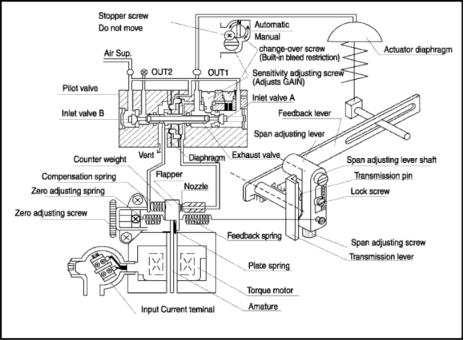
\includegraphics[width=\textwidth]
{Sections/2-DisenoEnsamblado/Images/PG-EPL.pdf}
	 \end{column}
	\end{columns}
}

\subsection*{Instrumentación}
\frame{ 
	\ifdebug
	\frametitle{Instrumentación\hfill{\color{red} \emph{F}}}
	\else
	\frametitle{Instrumentación}
	\fi

	
	Conocer \textbf{variables de interés} de la 
planta:
	
	\begin{itemize}
	 \item Nivel de los tanques $\Rightarrow$ DP cell
	 \item Caudal en la tubería de llenado $\Rightarrow$ Placa orificio
	 \item Presión en las tuberías $\Rightarrow$ Manómetros
	\end{itemize}
	
	\vspace{1cm}

	\begin{columns}
	 \begin{column}{.33\textwidth}
		\centering
	  	  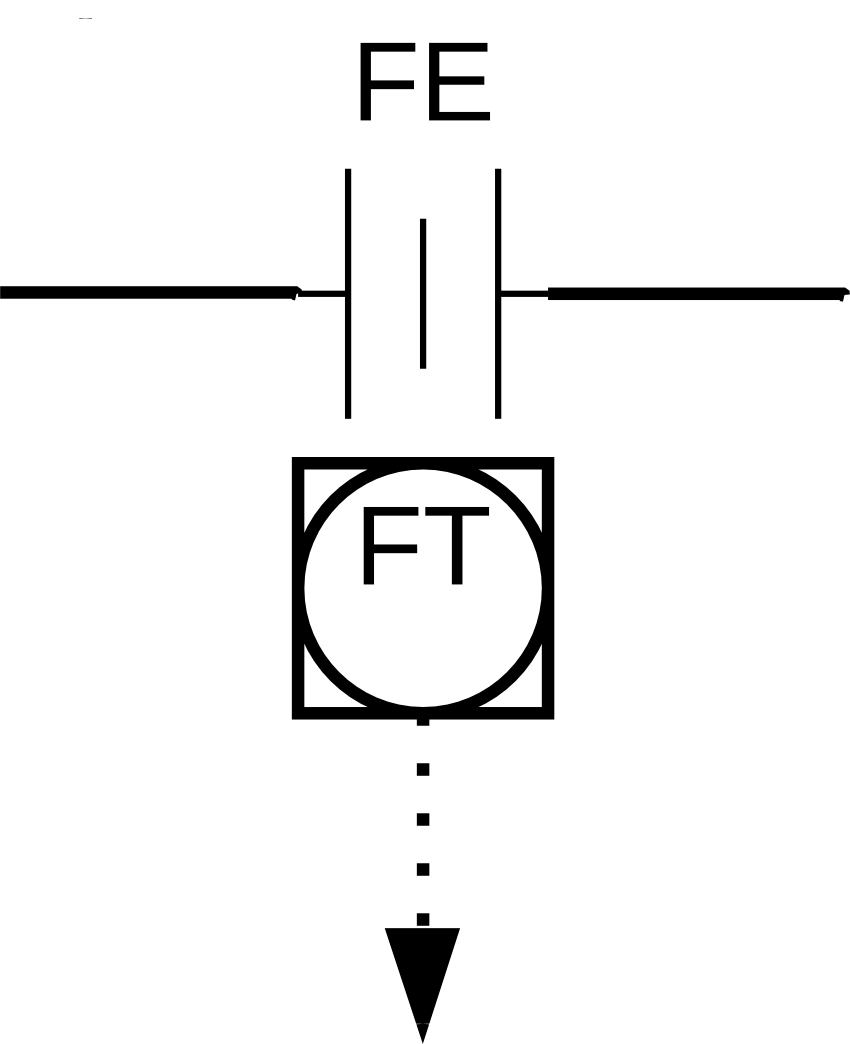
\includegraphics[height=.7\textwidth]
{Sections/2-DisenoEnsamblado/Images/FE-FTpyid.png}

	\footnotesize
	Placa orificio
	
	 \end{column}
	 \begin{column}{.33\textwidth}
		\centering
	  	  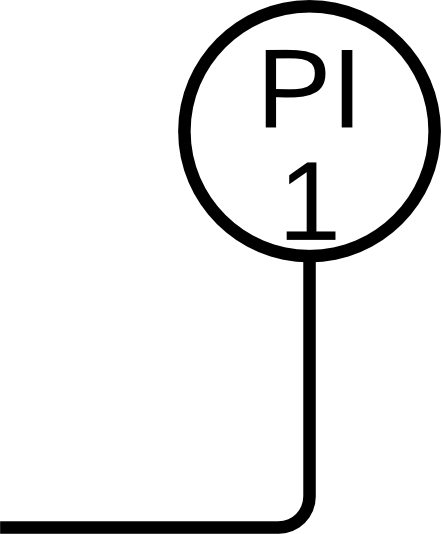
\includegraphics[height=.6\textwidth]
{Sections/2-DisenoEnsamblado/Images/PIpyid.png}
	
	\footnotesize
	Manómetros
	 \end{column}
	 \begin{column}{.33\textwidth}
	 \centering
	 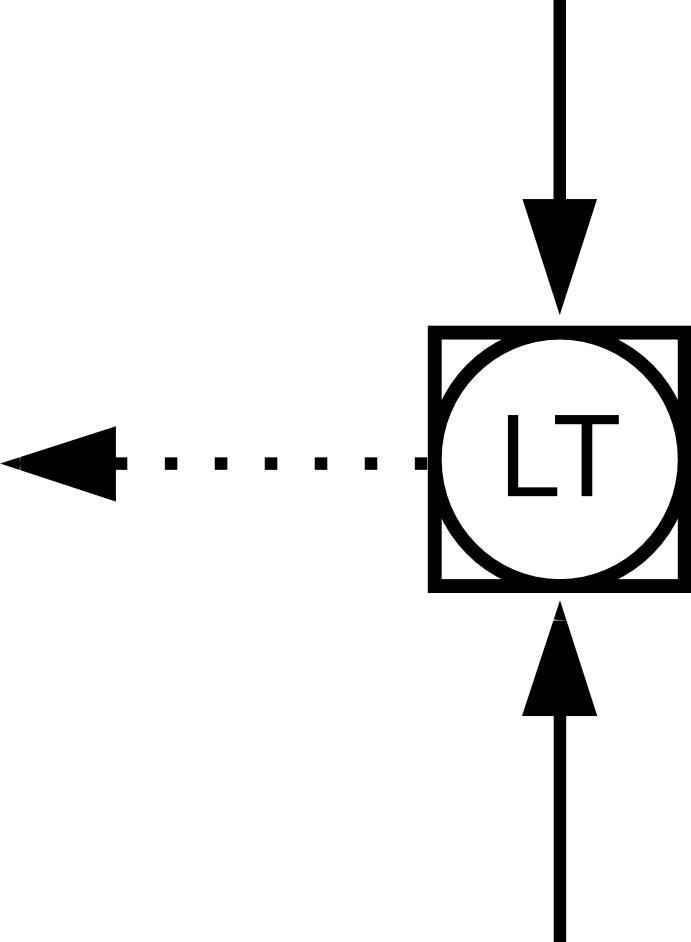
\includegraphics[height=.7\textwidth]
{Sections/2-DisenoEnsamblado/Images/DPpyid.png}

	\footnotesize
	DP cells
	 \end{column}
	\end{columns}

}

\frame{
	\ifdebug
	\frametitle{Manómetros\hfill{\color{red} \emph{F}}}
	\else
	\frametitle{Manómetros}
	\fi

	
	\textbf{Manómetro de tubo de Bourdón}
	
		\begin{itemize}
	  \item Valor de presión {\color{newcolor} instantánea}
	  \item Baja precisión
	  \item Permiten ecualizar la planta
	 \end{itemize}
	 \vspace{-.25cm}
	\begin{columns}[b]
	 \begin{column}{.5\textwidth}
	 \begin{center}
	  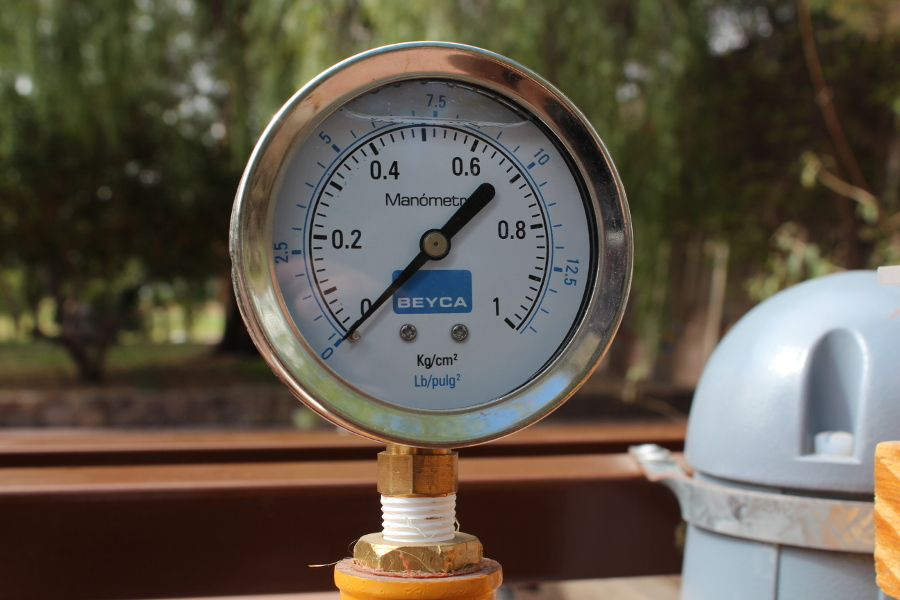
\includegraphics[height=.66\textwidth]
{Sections/2-DisenoEnsamblado/Images/manometro2.JPG}

\footnotesize

	Manómetro tubería de vaciado

	 \end{center}
	 \end{column}
	 \begin{column}{.5\textwidth}
	 
	 \begin{center}
	  
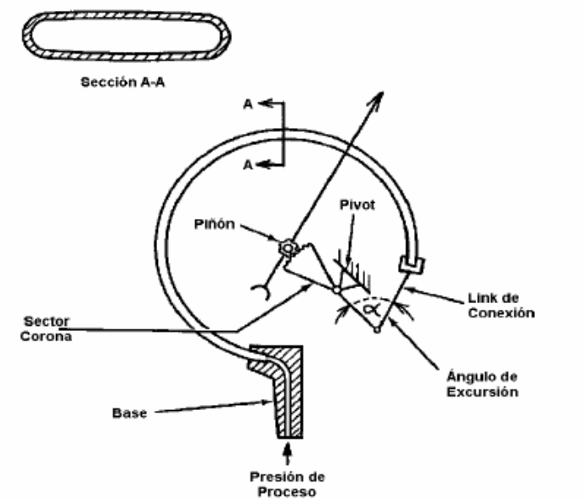
\includegraphics[height=.66\textwidth]
{Sections/2-DisenoEnsamblado/Images/manomBourdon.png}

\footnotesize

	Esquema de funcionamiento
	 \end{center}

	 \end{column}
	\end{columns}

}

\frame{
	\ifdebug
	\frametitle{DP Cell - celda de presión diferencial\hfill{\color{red} 
\emph{F}}}
	\else
	\frametitle{DP Cell - celda de presión diferencial}
	\fi
	
	Mide la \textbf{diferencia de presión} entre dos puntos
	
	\begin{columns}[t]
		\begin{column}{0.6\textwidth}
		\begin{center}
			 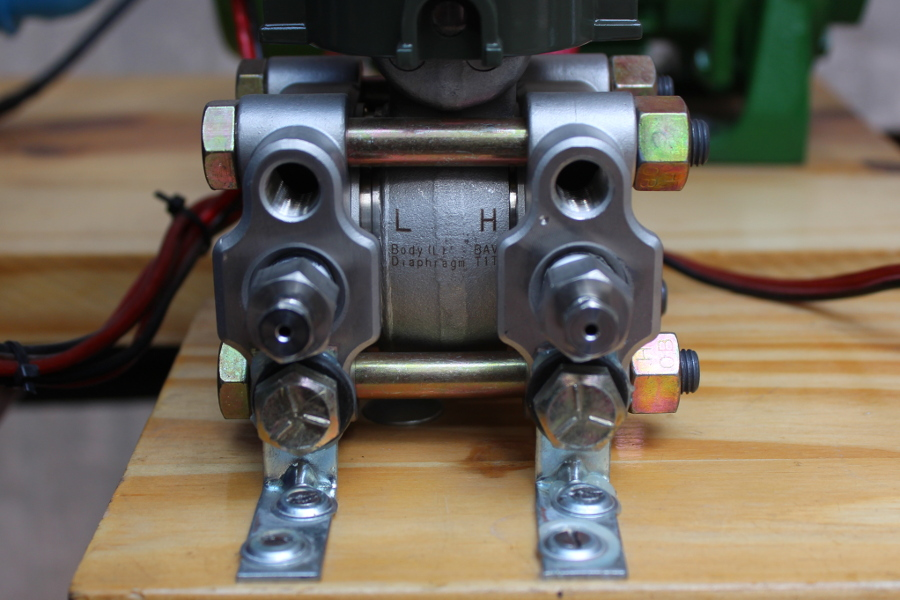
\includegraphics[width=\textwidth]
{Sections/2-DisenoEnsamblado/Images/dpcell2.JPG}

		\footnotesize

				Detalle tomas
			\end{center}
			\vspace{-.25cm}
			\begin{itemize}
			 \item Rango $0$ - $10000\,mmCa$
			 \item Output $4$ -$20\,mA$
			\end{itemize}
			
			
		\end{column}

		\begin{column}{0.4\textwidth}
			\begin{center}
				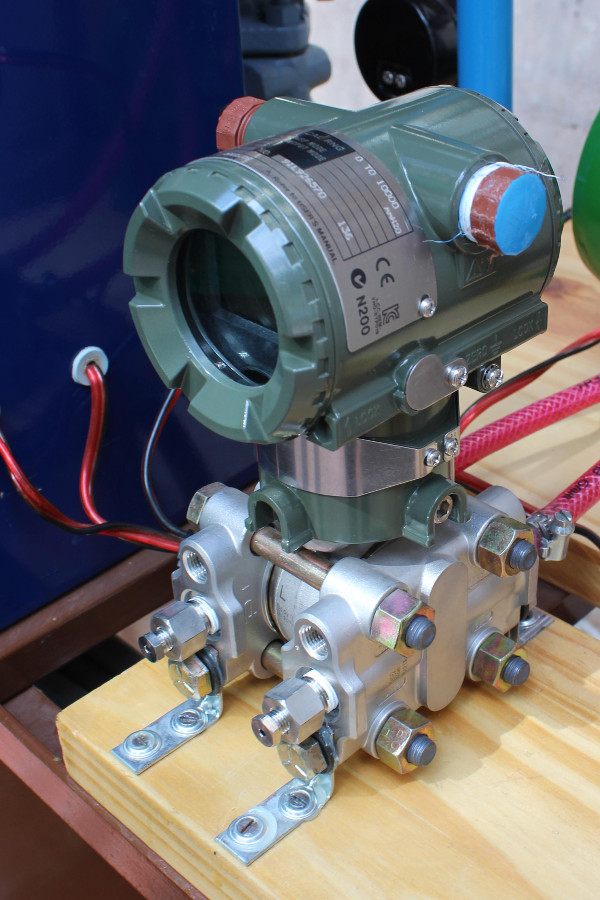
\includegraphics[width=.8\textwidth]
{Sections/2-DisenoEnsamblado/Images/dpcell1.JPG}
				\footnotesize

				DP Cell de caudal
			\end{center}
		\end{column}

	\end{columns}
}

\frame{
	\ifdebug
	\frametitle{Placa orificio\hfill{\color{red} \emph{F}}}
	\else
	\frametitle{Placa orificio}
	\fi

	
	\begin{center}
	  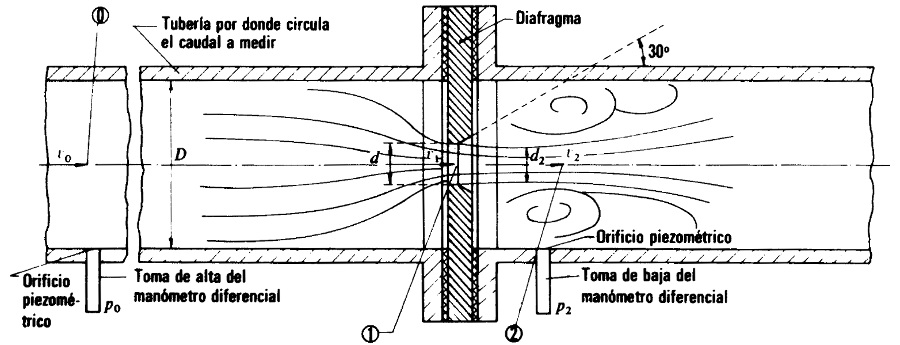
\includegraphics[width=.7\textwidth]
{Sections/2-DisenoEnsamblado/Images/placaOrif.png}

	\footnotesize
		Corte longitudinal placa orificio - tubería
	\end{center}

	
	Planteando Bernoulli...
	\vspace{-.5cm}
	\begin{center}
	  \begin{align*}
	  v_2^2 - v_0^2 &= 2\,g\,h_p 
	  \\
	    Q = \dfrac{C_v \, A_2}{\sqrt{1-\beta^4}}\, \sqrt{2 \, g \, 
h_p} \quad &\Rightarrow \quad Q \approx K\,\sqrt{h_p}
	  \end{align*}
	  \end{center}
	  
	  En este trabajo, constante $K$ se encuentra \textbf{experimentalmente}
}
